\documentclass[tikz,border=4pt]{standalone}
\usepackage{tikz}
\usetikzlibrary{arrows.meta}

\definecolor{rednode}{RGB}{227,27,35}

\begin{document}
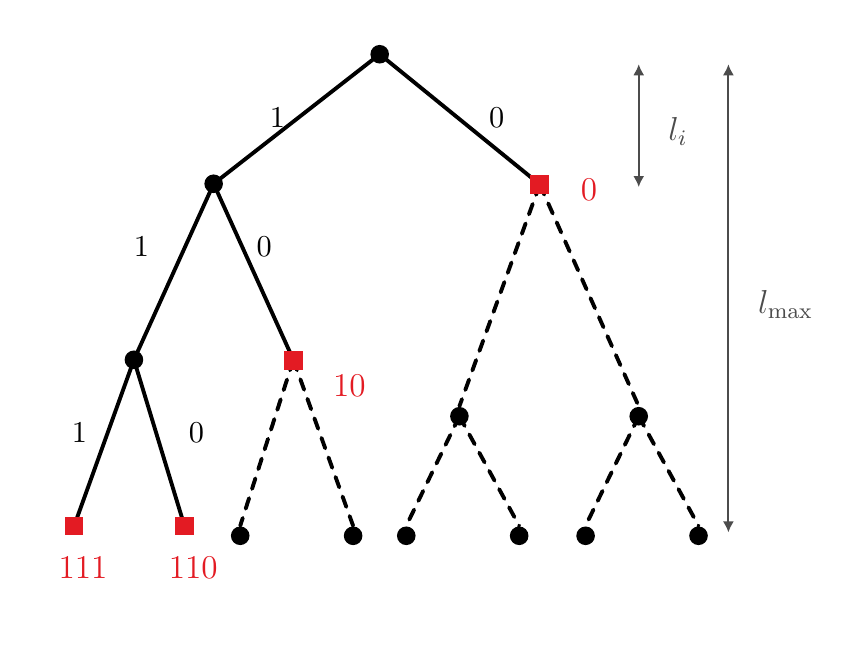
\begin{tikzpicture}[x=1pt,y=-1pt,scale=0.24,line cap=round,line join=round]
    \path[use as bounding box] (0,0) rectangle (1200,900);

    \draw[line width=1.4pt] (530,40) -- (280,235);
    \draw[line width=1.4pt] (530,40) -- (771,236);
    \draw[line width=1.4pt] (280,235) -- (160,500);
    \draw[line width=1.4pt] (280,235) -- (400,500);
    \draw[line width=1.4pt] (160,500) -- (70,750);
    \draw[line width=1.4pt] (160,500) -- (236,750);

    \draw[line width=1.4pt,dash pattern=on 4pt off 3.5pt] (400,500) -- (320,750);
    \draw[line width=1.4pt,dash pattern=on 4pt off 3.5pt] (400,500) -- (490,750);
    \draw[line width=1.4pt,dash pattern=on 4pt off 3.5pt] (771,236) -- (650,570);
    \draw[line width=1.4pt,dash pattern=on 4pt off 3.5pt] (771,236) -- (920,570);
    \draw[line width=1.4pt,dash pattern=on 4pt off 3.5pt] (650,585) -- (570,750);
    \draw[line width=1.4pt,dash pattern=on 4pt off 3.5pt] (650,585) -- (740,750);
    \draw[line width=1.4pt,dash pattern=on 4pt off 3.5pt] (920,585) -- (840,750);
    \draw[line width=1.4pt,dash pattern=on 4pt off 3.5pt] (920,585) -- (1010,750);

    \fill (530,40) circle[radius=14pt];
    \fill (280,235) circle[radius=14pt];
    \fill (160,500) circle[radius=14pt];
    \fill (320,765) circle[radius=14pt];
    \fill (490,765) circle[radius=14pt];
    \fill (650,585) circle[radius=14pt];
    \fill (920,585) circle[radius=14pt];
    \fill (570,765) circle[radius=14pt];
    \fill (740,765) circle[radius=14pt];
    \fill (840,765) circle[radius=14pt];
    \fill (1010,765) circle[radius=14pt];

    \fill[rednode] (757,222) rectangle (785,250);
    \fill[rednode] (386,487) rectangle (414,515);
    \fill[rednode] (56,736) rectangle (84,764);
    \fill[rednode] (222,736) rectangle (250,764);

    \draw[<->,>={Latex[length=4pt,width=4pt]},line width=0.7pt,black!70] (920,55) -- (920,240);
    \draw[<->,>={Latex[length=4pt,width=4pt]},line width=0.7pt,black!70] (1055,55) -- (1055,760);

    \node[anchor=base west,font=\fontsize{11}{11}\selectfont] at (350,150) {1};
    \node[anchor=base west,font=\fontsize{11}{11}\selectfont] at (680,150) {0};
    \node[anchor=base west,font=\fontsize{11}{11}\selectfont] at (145,345) {1};
    \node[anchor=base west,font=\fontsize{11}{11}\selectfont] at (330,345) {0};
    \node[anchor=base west,font=\fontsize{11}{11}\selectfont] at (52,625) {1};
    \node[anchor=base west,font=\fontsize{11}{11}\selectfont] at (228,625) {0};

    \node[anchor=base west,text=rednode,font=\fontsize{12}{12}\selectfont] at (32,830) {111};
    \node[anchor=base west,text=rednode,font=\fontsize{12}{12}\selectfont] at (198,830) {110};
    \node[anchor=base west,text=rednode,font=\fontsize{12}{12}\selectfont] at (445,555) {10};
    \node[anchor=base west,text=rednode,font=\fontsize{12}{12}\selectfont] at (818,260) {0};

    \node[anchor=base west,text=black!70,font=\fontsize{12}{12}\selectfont] at (950,170) {$l_i$};
    \node[anchor=base west,text=black!70,font=\fontsize{12}{12}\selectfont] at (1085,430) {$l_{\max}$};
\end{tikzpicture}
\end{document}
